\documentclass[xcolor=dvipsnames]{beamer}
\usepackage{xmpmulti}
\usepackage{comp2402}

%\usepackage[T1]{fontenc}
%\usepackage[sfdefault,black]{merriweather} %% Option 'black' gives heavier bold face 
%
%

%\usepackage{libris}
%\renewcommand*\familydefault{\sfdefault} %% Only if the base font of the document is to be sans serif
%\usepackage[T1]{fontenc}
%
% For source code:
\usepackage{minted}
\usepackage{mdframed}
\surroundwithmdframed{minted}



%\setbeamercovered{transparent}

% For aligning tables
\usepackage{array}

\newcommand{\mi}[1]{\multiinclude[<+>][start=1,format=pdf]{#1}}

\title{Computer Architecture Through Binary Searching}
\author{Pat Morin \\ (Joint Work with Paul Khuong)}
\date{Carleton University \\ AppNexus}


\begin{document}

\begin{frame}
  \titlepage
  \centerline{
    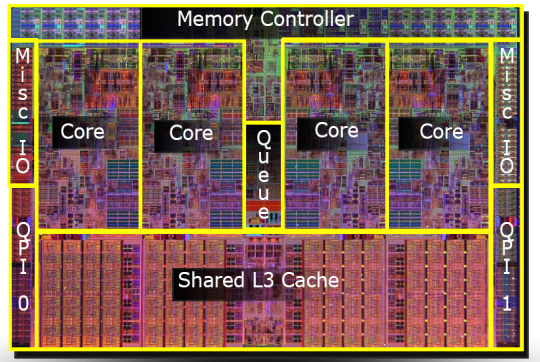
\includegraphics[height=1in]{images/nehalemdie}
    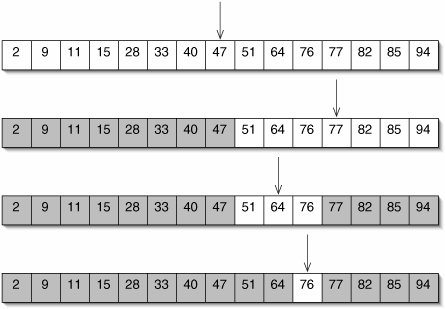
\includegraphics[height=1in]{images/binary-search}
    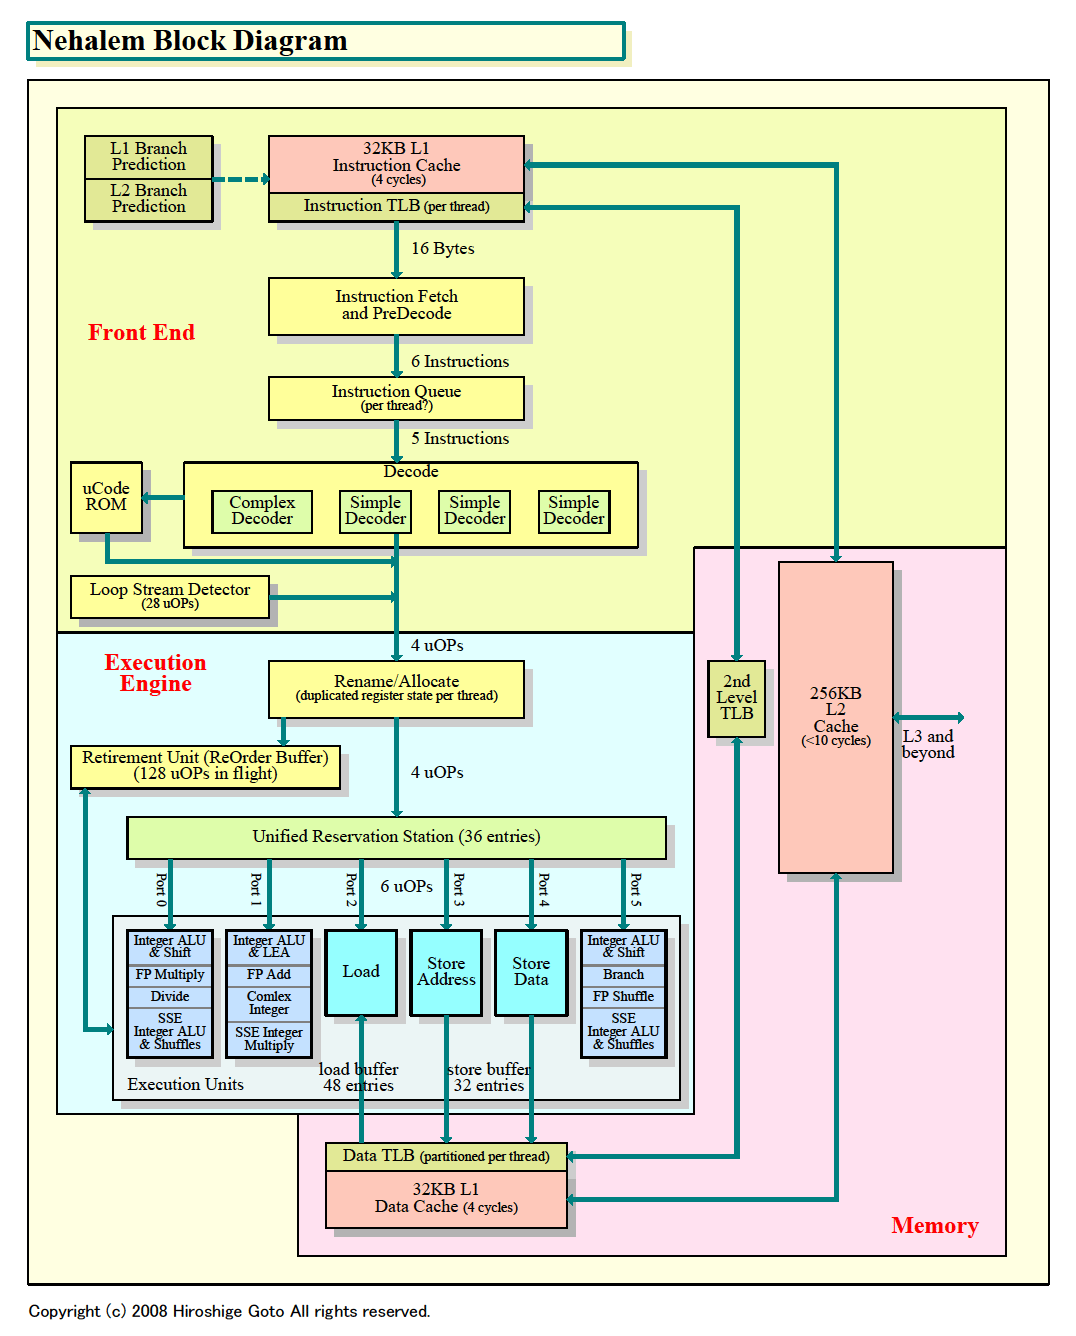
\includegraphics[height=1in]{images/nehalem-block}
  }
\end{frame}


\begin{frame}
  \setbeamercovered{transparent}
  \frametitle{Binary Search}
  \framesubtitle{Two Motivating Examples}

  \begin{itemize}
    \item<+-> Chromium Code Base (Google Chrome)
    \begin{itemize}
       \item \mintinline{c++}{std::upper_bound} called from 135 different locations
       \item Cookie handling, GUI layout, graphics and text rendering, video handling, and certificate management
       \item More than 1,000,000,000 users
    \end{itemize}
    \item<+->AppNexus real-time ad bidding engine
    \begin{itemize}
       \item Running 24/7 on 1500 machines
       \item 4,000,000 requests per second
       \item 10\% of CPU time spent on binary searching a few arrays
       \item 118,000,000 watt hours per year
    \end{itemize}
    \item<+->Plus thousands of other examples
  \end{itemize}
\end{frame}

\begin{frame}
  \frametitle{Microprocessor Architecture: Programmer's View}
  \framesubtitle{Von Neumann Architecture}

  \begin{center}
    \includegraphics[scale=0.85]{figs/programmers-view} 
  \end{center}
  
%  \begin{itemize}
%    \item<+->CPU repeatedly
%    \begin{itemize}
%      \item<+->Fetches an instruction (from RAM)
%      \item<+->Decodes the instruction
%      \item<+->Executes the instruction
%    \end{itemize}
%    \item<+->Instructions include:
%     \begin{itemize}
%      \item<+->Arithmetic operations on CPU registers
%      \item<+->Moving data between registers and RAM
%    \end{itemize}
%  \end{itemize}
  
\end{frame}


\begin{frame}
  \frametitle{Binary Search}
  \framesubtitle{The Classic Data Structure/Query Algorithm}

  \begin{center}
    \mi{figs/binary-search-example}
  \end{center}
  \begin{itemize}[<10->]
    \item Finds 8 or finds where 8 should be
  \end{itemize}

\end{frame}



\begin{frame}[fragile]
  \frametitle{Binary Search}
  \framesubtitle{Branchy Code}

{\small
\begin{minted}{c++}
template<typename T, typename I>
I sorted_array<T,I>::branchy_search(T x) const {
    I lo = 0, hi = n;
    while (lo < hi) {
        I m = (lo + hi) / 2;
        if (x < a[m]) {
            hi = m;
        } else if (x > a[m]) {
            lo = m+1;
        } else {
            return m;
        }
    }
    return hi;
}
\end{minted}
}
\end{frame}

\begin{frame}[fragile]
  \frametitle{Binary Search: Analysis}

  \begin{itemize}
    \item Each iteration terminates or 
      reduces \mintinline{c++}{hi-lo} by a factor of 2
    \item $\therefore$ at most $\log_2 n$ iterations
    \item Doubling the size of the array adds only one more iteration
  \end{itemize}
\end{frame}

\begin{frame}
  \frametitle{Branchy Binary Search: Experiments}
  \begin{center}
    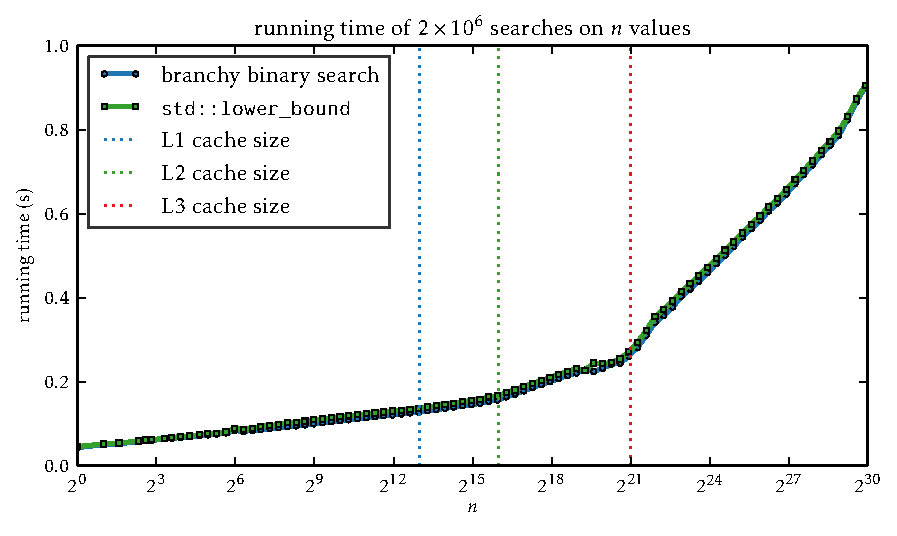
\includegraphics{graphs/sorted-i}
  \end{center}
\end{frame}

\begin{frame}[fragile]
  \frametitle{Binary Search}
  \framesubtitle{Branchy Assembly Code}

%\vspace{-2em}
\tiny
%\resizebox{\textwidth}{\textheight}{
\begin{minted}{nasm}
       .cfi_startproc
       movq    8(%rdi), %rax
       xorl    %ecx, %ecx
       movq    (%rdi), %r8
       cmpq    %rcx, %rax
       jbe     .L5                 ; quit if lo == hi
.L11:  leaq    (%rcx,%rax), %rdx   ; top of while loop
       shrq    %rdx
       movl    (%r8,%rdx,4), %edi  ; load a[m]
       cmpl    %edi, %esi          ; compare a[m] and x
       jnb    .L3                  ; jump if a[m] <= x
 .L8:  cmpq    %rdx, %rcx          ; a[m] > x, search first half
       movq    %rdx, %rax
       jnb     .L5
       addq    %rcx, %rdx          ; lo + hi
       shrq    %rdx                ; (lo + hi) / 2
       movl    (%r8,%rdx,4), %edi  ; load a[m]
       cmpl    %edi, %esi          ; compare a[m] and x
       jb      .L8                 ; jump if a[m] > x
 .L3:  cmpl    %edi, %esi          ; here a[m] <= x
       jbe     .L7                 ; quit if a[m] == x
       leaq    1(%rdx), %rcx
       cmpq    %rcx, %rax
       ja      .L11                ; back to top, if lo < hi
 .L5:  rep ret
 .L7:  movq    %rdx, %rax
       ret
       .cfi_endproc
\end{minted}
%}

\end{frame}

\begin{frame}
   \frametitle{Binary Search is Optimal}

   \begin{itemize}
     \item Binary search is ``optimal''
     \item It does the fewest number of comparisons possible
     \item But are comparisons really the most expensive thing we do?
   \end{itemize}
\end{frame}

\begin{frame}
   \frametitle{The Instruction Pipeline}

   \begin{center}
      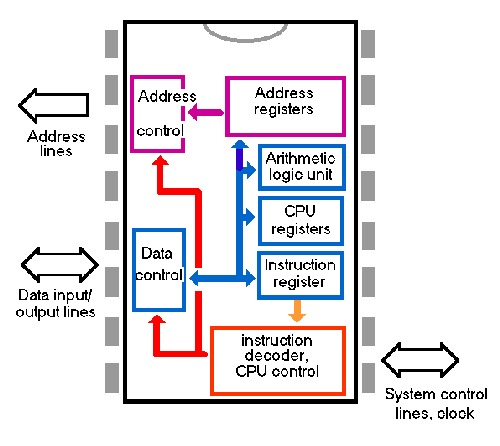
\includegraphics[width=.3\textwidth]{images/micro3c}
      \multiinclude[<+>][start=1,format=pdf,graphics={width=.7\textwidth}]{figs/pipeline}
   \end{center}
   \vspace{-1em}
   \begin{itemize}
     \item<4->Guess wrong and we have to flush the whole pipeline!
     \item<5->May take 20--24 cycles!
   \end{itemize}
\end{frame}


\begin{frame}
   \frametitle{Branch-Free Binary Search}

   \begin{itemize}
       \item Branchy binary search will guess 
                wrong nearly 50\% of the time.
       \item Solution: Eliminate branching with conditional moves (\texttt{\color{blue}cmov})
   \end{itemize}
\end{frame}


\begin{frame}[fragile]
   \frametitle{Branch-Free Binary Search}
   \framesubtitle{C++ Code}
\begin{minted}{c++}
I sorted_array<T,I>::branchfree_search(T x) const {
  const T *base = a;
  I n = this->n;
  while (n > 1) {
    const I half = n / 2;
    base = (base[half] < x) ? &base[half] : base;
    n -= half;
  }
  return (*base < x) + base - a;
}
\end{minted}
\end{frame}

\begin{frame}[fragile]
   \frametitle{Branch-Free Binary Search}
   \framesubtitle{Assembly Code}

\tiny
\begin{minted}{nasm}
  .cfi_startproc
  movq    8(%rdi), %rdx       ; move n into rdx
  movq    (%rdi), %r8         ; move a into r8
  cmpq    $1, %rdx            ; compare n and 1
  movq    %r8, %rax           ; move base into rax
  jbe    .L2                  ; quit if n <= 1
.L3:
  movq    %rdx, %rcx          ; put n into rcx
  shrq    %rcx                ; rcx = half = n/2
  leaq    (%rax,%rcx,4), %rdi ; load &base[half] into rdi
  cmpl    %esi, (%rdi)        ; compare x and base[half]
  cmovb   %rdi, %rax          ; set base = &base[half] if x > base[half]
  subq    %rcx, %rdx          ; n = n - half
  cmpq    $1, %rdx            ; compare n and 1
  ja      .L3                 ; keep going if n > 1
.L2:
  cmpl    %esi, (%rax)        ; compare x to *base
  sbbq    %rdx, %rdx          ; set dx to 00..00 or 11...11
  andl    $4, %edx            ; set dx to 0 or 4 
  addq    %rdx, %rax          ; add dx to base
  subq    %r8, %rax           ; compute base - a (* 4)
  sarq    $2, %rax            ; (divide by 4)
  ret
  .cfi_endproc
\end{minted}
\end{frame}

\begin{frame}[fragile]
   \frametitle{Branch-Free Binary Search}
   \framesubtitle{Performance}

   \begin{center}
     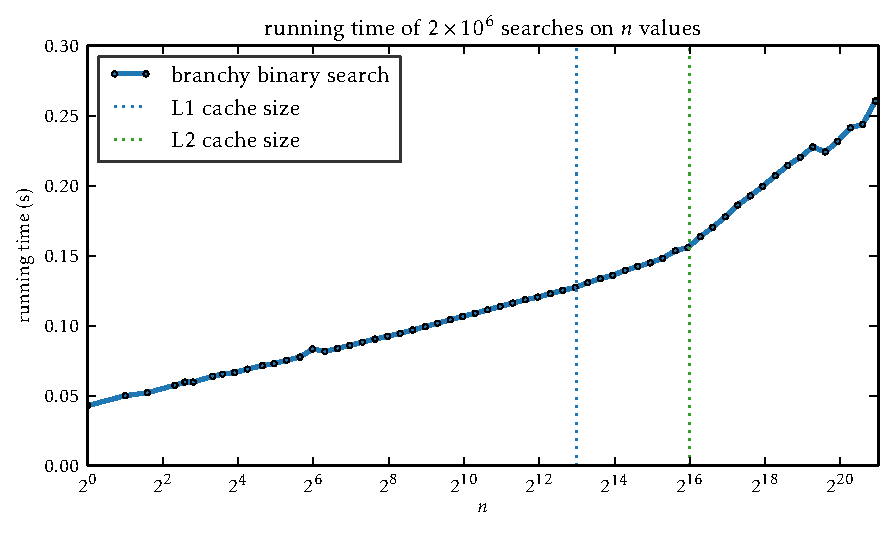
\includegraphics{graphs/sorted-ii}
   \end{center}
\end{frame}


\begin{frame}
   \frametitle{Binary Search is Optimal}

   \begin{itemize}
     \item Binary search is ``optimal''
     \begin{itemize}
       \item It does the fewest number of comparisons possible
       \item Branch-free version makes no branch mispredictions
     \end{itemize}
     \item Anything else we need to worry about?
   \end{itemize}
\end{frame}


\begin{frame}
   \frametitle{The Memory Hierarchy}

   \begin{center}
     \only<+>{\includegraphics[scale=0.85]{figs/programmers-view}}%
     \only<+->{\includegraphics[scale=0.85]{figs/caches}}
   \end{center}
   \begin{itemize}
     \item<+->Sizes: RAM (GB), L3 (MB), L2 (100's of KB), L1 (KB)
     \item<+->Speeds: RAM (100 cycles), L3 (40 cycles), L2 (10 cycles), L1 (4 cycles)
   \end{itemize}
   
\end{frame}

\begin{frame}
   \frametitle{Branch-Free Binary Search}
   \framesubtitle{Performance}

   \begin{center}
     \only<+>{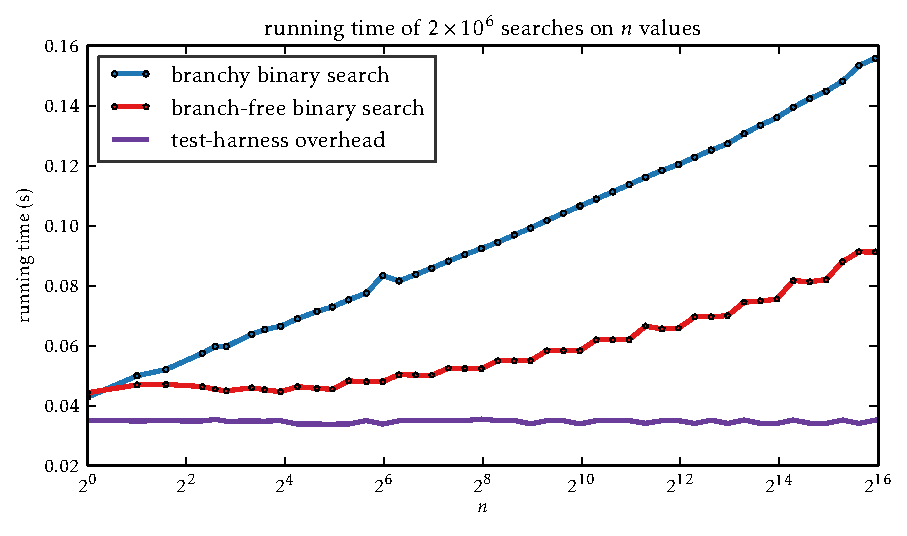
\includegraphics{graphs/sorted-iii}}%
     \only<+>{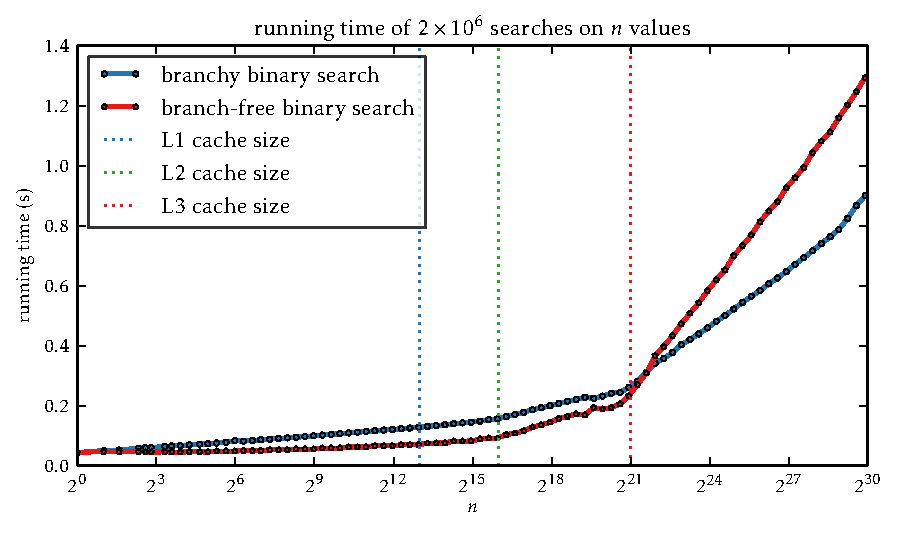
\includegraphics{graphs/sorted-iv}}%
     \only<+>{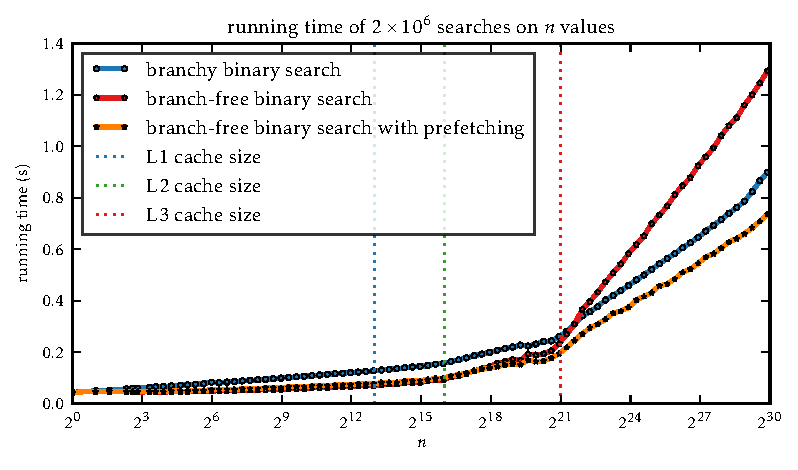
\includegraphics{graphs/sorted-v}}%
     \only<+>{\includegraphics{graphs/sorted-vi}}%
   \end{center}
\end{frame}

\begin{frame}[fragile]
   \frametitle{Branchy versus Branch-Free Binary Search}
   \framesubtitle{Performance}

   \begin{tabular}{m{.48\textwidth}m{.48\textwidth}}
\tiny
 \begin{minted}{c++}
template<typename T, typename I>
I sorted_array<T,I>::branchy_search(T x) {
    I lo = 0, hi = n;
    while (lo < hi) {
        I m = (lo + hi) / 2;
        if (x < a[m]) {
            hi = m;
        } else if (x > a[m]) {
            lo = m+1;
        } else {
            return m;
        }
    }
    return hi;
}
\end{minted}
&
     \includegraphics[scale=0.5]{graphs/sorted-vi}
\end{tabular}
\begin{itemize}
  \item Branch-prediction is wrong $50\%$ the time
     \begin{itemize}
       \item Causes costly pipeline flush
     \end{itemize}
  \item Branch-prediction is right $50\%$ the time
      \begin{itemize}
       \item Puts memory subsystem to work loading from memory
     \end{itemize}
  \item RAM latency $\approx100$ cycles, pipeline latency $\approx 20$ cycles
\end{itemize}
\end{frame}

\begin{frame}[fragile]
   \frametitle{Branch-Free Binary Search with Prefetching}
   \framesubtitle{The best of both worlds}

   {\tiny
   \begin{minted}{c++}
template<typename T, typename I>
I sorted_array<T,I>::_branchfree_search(T x) const {
    const T *base = a;
    I n = this->n;
    while (n > 1) {
        I half = n / 2;
        __builtin_prefetch(base + half/2, 0, 0);
        __builtin_prefetch(base + half + half/2, 0, 0);
        base = (base[half] < x) ? base+half : base;
        n -= half;
    }
    return (*base < x) + base - a;
}
   \end{minted}
   }
   \includegraphics[width=.5\textwidth]{graphs/sorted-vii}
   \includegraphics[width=.5\textwidth]{graphs/sorted-viii}

\end{frame}

\begin{frame}[fragile]
   \frametitle{With and Without Prefetching}

   \begin{center}
      \only<+->{\includegraphics[width=.98\textwidth]{figs/timeline-binary-search}}
   \end{center}
   \begin{itemize}[<+->]
     \item Processor and memory subsystem work in \emph{parallel}
     \item Memory subsystem has its own pipeline
   \end{itemize}
\end{frame}

\begin{frame}
  \title{Array Layouts for Comparison-Based Searching}
  \titlepage
  \centerline{
    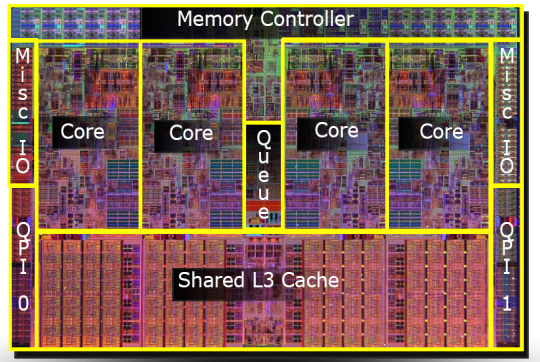
\includegraphics[height=1in]{images/nehalemdie}
    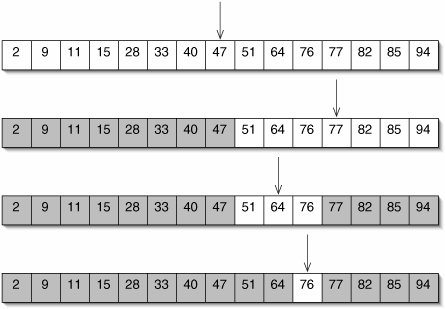
\includegraphics[height=1in]{images/binary-search}
    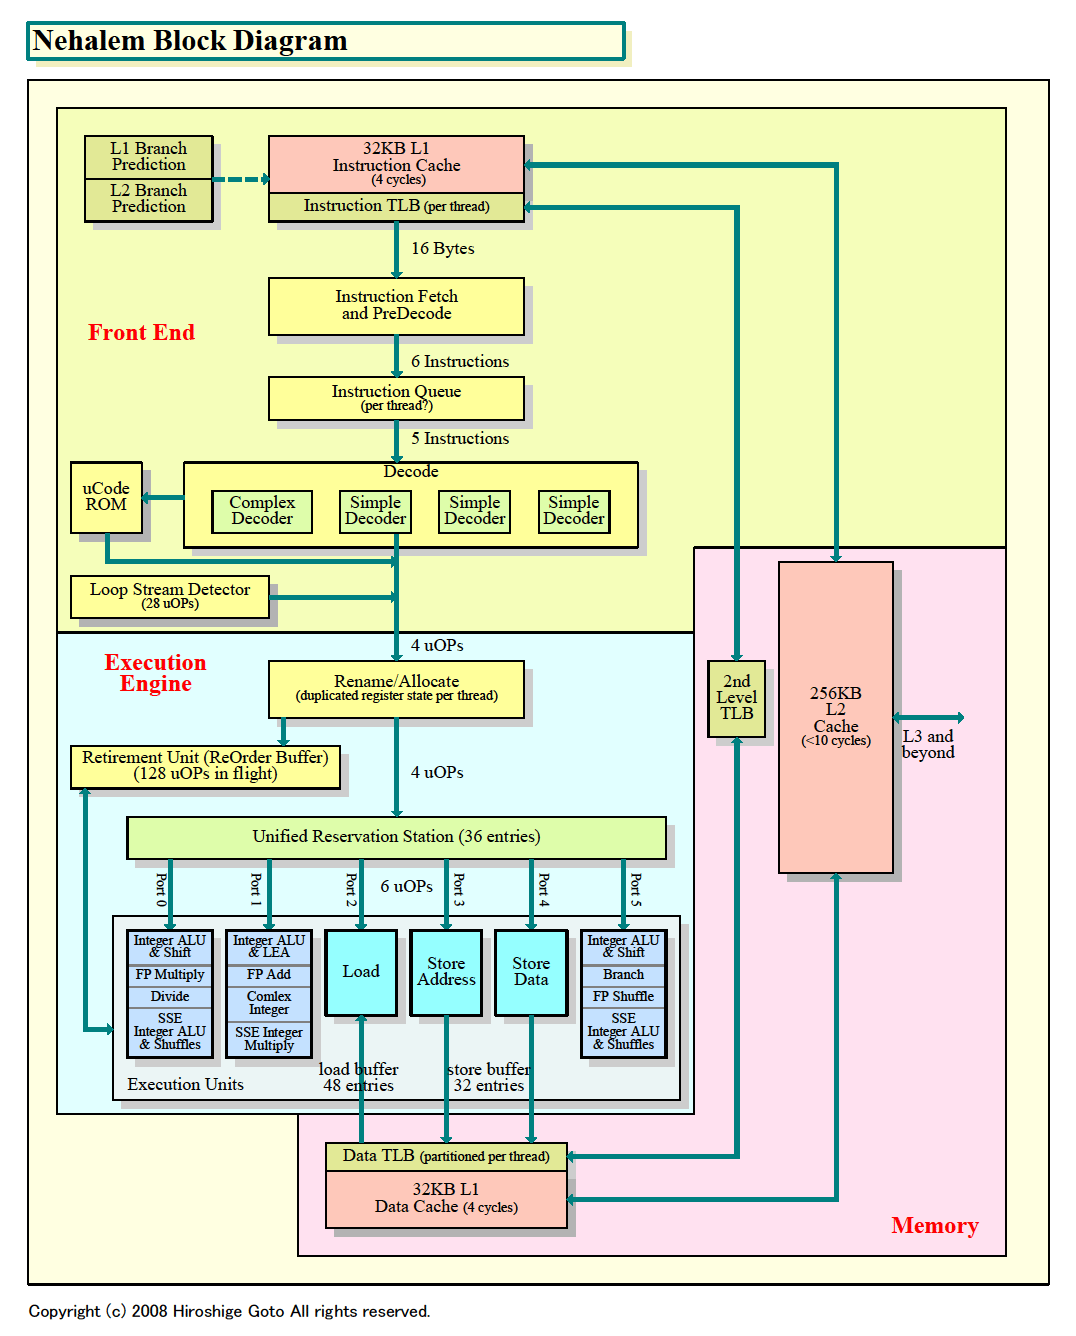
\includegraphics[height=1in]{images/nehalem-block}
  }
\end{frame}

\begin{frame}[fragile]
   \frametitle{The Story So Far}

   \begin{itemize}
      \item<+->Long processor pipelines require branch prediction
               for performance
      \begin{itemize}
         \item<+->Branch mispredictions are expensive (20--25 cycles)
         \item<+->Branches can sometimes be avoided using 
                  \mintinline{nasm}{cmov}
      \end{itemize}
      \item<+->Memory is a hierarchy
      \begin{itemize}
         \item<+->L1, L2, L3, RAM\only<+->{, Disk}\only<+->{, Cloud}%
            \only<+->{,\ldots}
         \item<+->Memory subsystem \emph{prefetches} as soon as it can
         \item<+->We can prefetch explicitly (using \mintinline{c++}{__builtin_prefetch})
         \item<+->We can prefetch implicitly (using branchy code)
      \end{itemize}
      \item<+->Long pipelines and memory hierarchy interact in surprising
               ways
   \end{itemize}
\end{frame}


\begin{frame}
   \frametitle{Binary Search is Optimal}

   \begin{itemize}[<+->]
     \item Binary search is optimal 
     \begin{itemize}
       \item It does the fewest number of comparisons possible
       \item Branch-free version makes no branch mispredictions
       \item Branch-free prefetching version makes no branch mispredictions\\
        \centerline{\includegraphics[width=.5\textwidth]{graphs/sorted-viii}}
     \end{itemize}
     \item Its interaction with the cache is non-optimal
   \end{itemize}
\end{frame}

\begin{frame}
   \frametitle{Cache Lines}

   \begin{itemize}
      \item<+-> RAM and caches are organized into \emph{lines}
      \begin{itemize}
        \item<+-> 64 bytes wide, can store
        \begin{itemize}
        \item 16 32-bit quantities (\mintinline{c++}{int}/\mintinline{c++}{int32_t}/\mintinline{c++}{float})
        \item 8 64-bit quantities (\mintinline{c++}{long long}/\mintinline{c++}{int64_t}/\mintinline{c++}{double})
        \item 4 128-bit quantities (\mintinline{c++}{int128_t}/\mintinline{c++}{quad})
        \end{itemize}
      \end{itemize}
      \item<+-> Accessing a single word of RAM loads an entire line
         into the cache hierarchy ($B$ items)
   \end{itemize}
   \begin{center}
      \only<1-3>{\includegraphics{figs/cache-lines-1}}%
      \only<4->{\includegraphics{figs/cache-lines-2}}
   \end{center}
   \begin{itemize}
        \item<+->Accessing a single item from RAM costs nearly as much as accessing a whole cache line
   \end{itemize}
\end{frame}

\begin{frame}
   \frametitle{Binary Search is Bad for Locality}
   \framesubtitle{Actually, sorted order is bad}

   \begin{itemize}
      \item<+->Binary search loads a lot of data that it never looks at
   \end{itemize}
   \begin{center}
      \mi{figs/binary-search-bad}%
   \end{center}
   \begin{itemize}
      \item<13->Loads $\log n - \log B$ cache lines
      \item<14->Example: $n =2^{30}$, $B=16$
      \begin{itemize}
          \item<15->$\log n - \log B=26$
          \item<16->Binary search inspects 30 values in 26 different cache lines
      \end{itemize}
      \item<17->To do better we need a different layout (not sorted)
   \end{itemize}
\end{frame}


\begin{frame}
   \frametitle{B-Trees}
   \framesubtitle{Bayer and McCreight 1972}

   \begin{itemize}
      \item<+->Use a $(B+1)$-ary search tree
      \item<+->Stores $B$ items per node (node fits neatly into cache line)
   \end{itemize}
   \begin{center}
      \only<1-2>{\includegraphics[width=.8\textwidth]{figs/btree-1}}%
      \only<3>{\includegraphics[width=.8\textwidth]{figs/btree-2}}%
      \only<4>{\includegraphics[width=.8\textwidth]{figs/btree-3}}%
      \only<5->{\includegraphics[width=.8\textwidth]{figs/btree-4}}%
   \end{center}
   \begin{itemize}
      \item<+->Lay nodes out into an array
   \end{itemize}
\end{frame}
 

\begin{frame}
   \frametitle{B-Tree Search}

   \begin{center}
      \mi{figs/btree-search}
   \end{center}
   \begin{itemize}
      \item<13->Accesses $\lceil\log_{B+1} n\rceil=\left\lceil\frac{\log n}{\log(B+1)}\right\rceil$ cache lines
      \item<14->Does binary search within each cache line: $\lceil\log(B+1)\rceil$ comparisons
      \item<15->Example: $n=2^{30}$, $B=16$
      \begin{itemize}
         \item<16->$\lceil\log_{B+1} n\rceil = 8$ cache lines per search
         \item<17->Compared to 26 cache lines with binary search
      \end{itemize}
   \end{itemize}
\end{frame}

\begin{frame}
   \frametitle{B-Tree Search}
   \framesubtitle{Performance}
   \only<+>{
      \begin{center}
         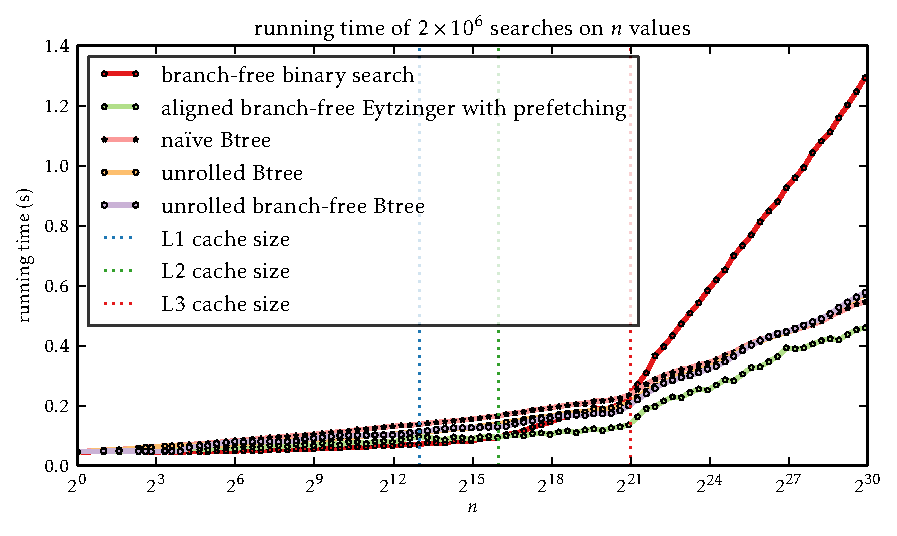
\includegraphics[height=.6\textheight]{graphs/btree-i} 
            \newline Good!
      \end{center}
   }
   \only<+>{
     \begin{tabular}{m{.2\textwidth}m{.75\textwidth}}
        \begin{center}
           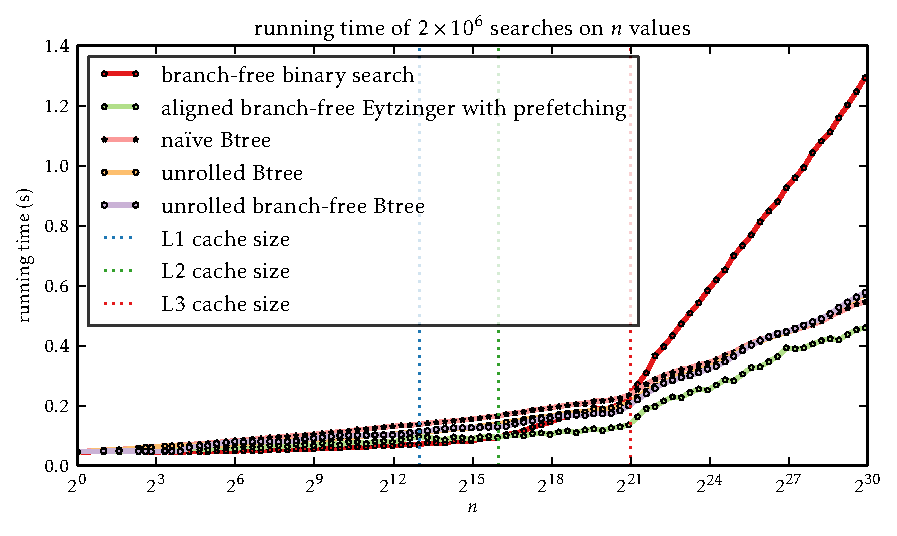
\includegraphics[width=.2\textwidth]{graphs/btree-i} 
             \newline Good!
        \end{center} &
        \begin{center}
           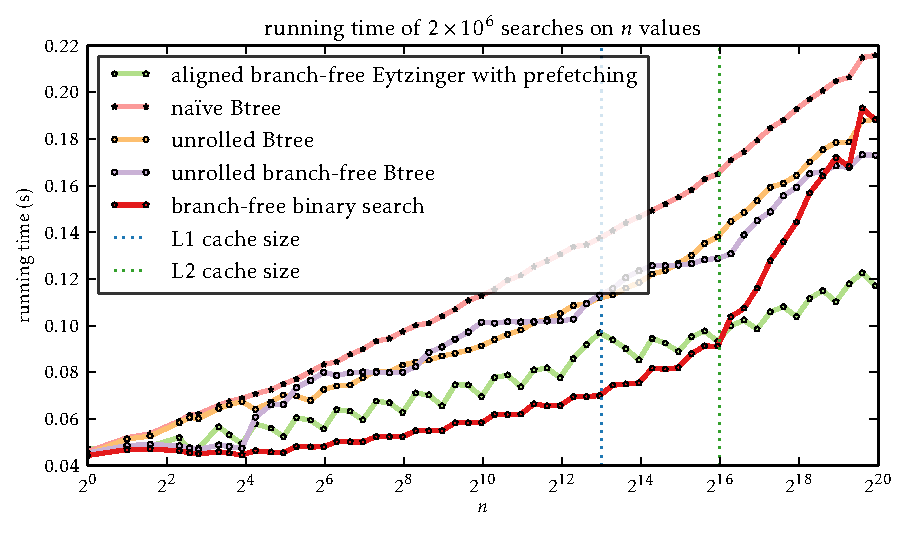
\includegraphics[width=.73\textwidth]{graphs/btree-ii} 
             \newline Bad!
        \end{center}
     \end{tabular}
   }
\end{frame}

\begin{frame}
   \frametitle{B-Tree Search Problems}
   \framesubtitle{Why are B-Trees so slow?}
    
   \begin{itemize}[<+->]
      \item Internal binary search has $B+1$ possible outcomes:
      \begin{itemize}
        \item For $B=16$, 
                  $\lceil\log(B+1)\rceil = \lceil 4.08\rceil = 5$ comparisons per node
      \end{itemize}
      \item Big jump in search time for each new level 
      \begin{itemize}
        \item Example: $n=2^{10}$, $B=16$, 
                  $\lceil\log_{B+1}n\rceil = \lceil 2.44\rceil = 3$ levels
        \item $3\times 5 = 15$ comparisons (versus 10 for binary search)
      \end{itemize}
      \item B-tree code is long, complicated, requires extra bookkeeping
   \end{itemize}
   \begin{tabular}{m{.45\textwidth}m{.45\textwidth}}
      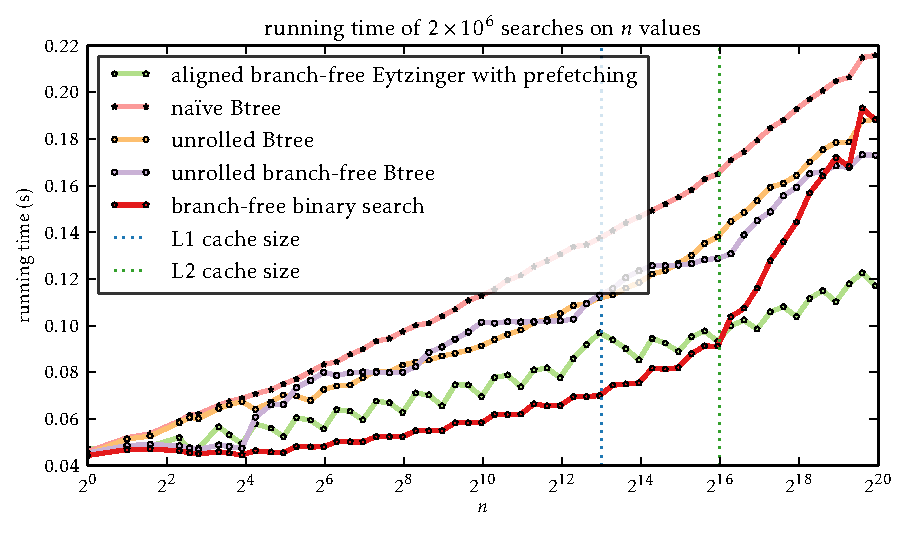
\includegraphics[width=.45\textwidth]{graphs/btree-ii}
     & \includegraphics[width=.45\textwidth]{figs/btree-4}
   \end{tabular}
   
\end{frame}


\begin{frame}
   \frametitle{B-Trees and Binary Search are Optimal}

   \begin{itemize}
     \item<+-> Binary search is ``optimal''
     \begin{itemize}
       \item It does the fewest number of comparisons possible
       \item Branch-free version makes no branch mispredictions
       \item But not cache-friendly!
     \end{itemize}
     \item<+-> B-Trees are ``optimal''
     \begin{itemize}
       \item They access the fewest number of cache lines possible
       \item But do more comparisons than necessary!
       \item Search code is more complicated!
     \end{itemize}
     \item<+-> What next?
   \end{itemize}
\end{frame}

\begin{frame}
   \frametitle{Beating B-Trees and Binary Search}

   \only<+->{Things we know:}
   \begin{enumerate}[<+->]
      \item Branch misprediction is costly
      \item Memory is chunked into 64 byte cache lines
      \item Memory subsystem can prefetch at the same time we compute
   \end{enumerate}
   \begin{itemize}[<+->]
      \item B-Trees take advantage of 1 \& 2.
      \item B-Trees don't take advantage of 3.
      \item B-Tree problems:
      \begin{itemize}
          \item When $B$ is a power of 2, $B+1$ is not
          \item Extra bookkeeping during search is expensive
      \end{itemize}
   \end{itemize}
\end{frame}

\begin{frame}
   \frametitle{The Eytzinger Layout}
   \framesubtitle{A.K.A. 1-trees}
  
   \begin{center}
      \only<+>{\includegraphics[width=.85\textwidth]{figs/eytzinger-1}}%
      \only<+>{\includegraphics[width=.85\textwidth]{figs/eytzinger-2}}%
      \only<+>{\includegraphics[width=.85\textwidth]{figs/eytzinger-3}}%
      \only<+->{\includegraphics[width=.85\textwidth]{figs/eytzinger-4}}
   \end{center} 
   \begin{itemize}
     \item Children of $i$ are at $2i+1$ and $2i+2$.
   \end{itemize}
\end{frame}

\begin{frame}[fragile]
   \frametitle{Branch-Free Eytzinger Search}

{\small 
\begin{minted}{c++}
template<typename T, typename I>
I eytzinger_array<T,I>::_branchfree_search(T x) const {
    I i = 0;
    while (i < n) {
        i = (x <= a[i]) ? (2*i + 1) : (2*i + 2);
    }
    I j = (i+1) >> __builtin_ffs(~(i+1));
    return (j == 0) ? n : j-1;
}
\end{minted} 
}
\end{frame}

\begin{frame}[fragile]
\frametitle{Branch-Free Eytzinger Search}

{\tiny
\begin{minted}{nasm}
    .cfi_startproc
    movq    8(%rdi), %rax
    xorl    %edx, %edx
    jmp     .L58
.L61:                            ; top of while loop
    movq    (%rdi), %rcx
    leaq    1(%rdx,%rdx), %r8
    leaq    2(%rdx,%rdx), %r9
    cmpl    %esi, (%rcx,%rdx,4)
    movq    %r8, %rdx
    cmovb   %r9, %rdx
.L58:
    cmpq    %rax, %rdx
    jb      .L61                 ; jump to top of while loop
    leal    1(%rdx), %ecx
    movl    $-1, %esi
    notl    %ecx
    bsfl    %ecx, %ecx
    cmove   %esi, %ecx
    addq    $1, %rdx
    addl    $1, %ecx
    shrq    %cl, %rdx
    leaq    -1(%rdx), %rcx
    testq   %rdx, %rdx
    cmovne  %rcx, %rax
    ret
    .cfi_endproc
\end{minted}
}
\end{frame}


\begin{frame}
\frametitle{Eytzinger Search}
\framesubtitle{Can we make it cache-friendly?}

\begin{center}
   \only<1>{\includegraphics[width=.9\textwidth]{figs/eytzinger-cache-1}}%
   \only<2>{\includegraphics[width=.9\textwidth]{figs/eytzinger-cache-2}}%
   \only<3->{\includegraphics[width=.9\textwidth]{figs/eytzinger-cache-3}}%
\end{center}
\begin{itemize}
   \item<4-> All 16 great-great granchdildren of $i$ are in the same cache line
   \item<5-> We can prefetch them 4 levels before they're needed
\end{itemize}
\end{frame}

\begin{frame}[fragile]
   \frametitle{Branch-Free Eytzinger Search with Prefetching}

{\small 
\begin{minted}{c++}
template<typename T, typename I>
I eytzinger_array<T,I>::_branchfree_search(T x) const {
    I i = 0;
    while (i < n) {
        __builtin_prefetch(a+(multiplier*i + offset));
        i = (x <= a[i]) ? (2*i + 1) : (2*i + 2);
    }
    I j = (i+1) >> __builtin_ffs(~(i+1));
    return (j == 0) ? n : j-1;
}
\end{minted} 
}
\end{frame}


\begin{frame}
  \frametitle{Eytzinger Performance}

  \begin{center}
    \only<+>{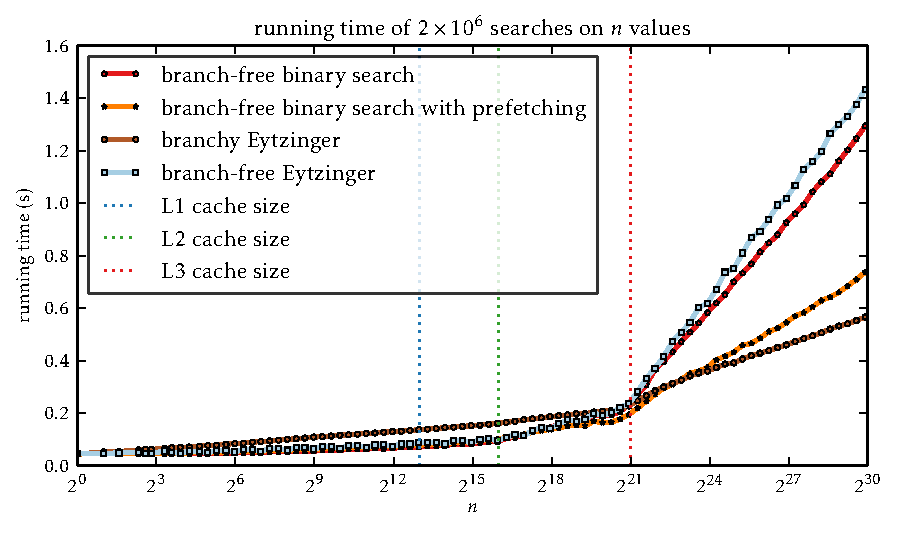
\includegraphics{graphs/eytzinger-i}}
    \only<+->{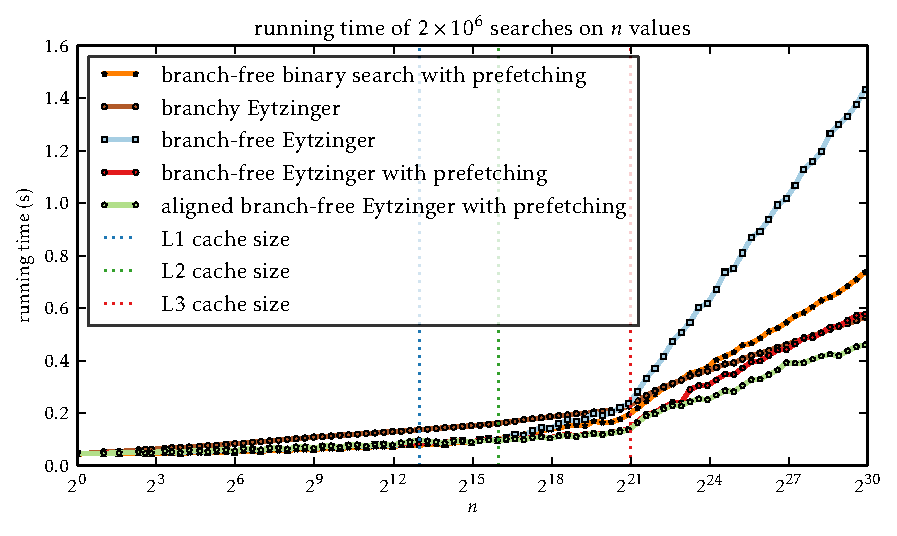
\includegraphics{graphs/eytzinger-ii}}
  \end{center}
\end{frame}

\begin{frame}
  \frametitle{Eytzinger versus B-Tree}

  \begin{center}
    \includegraphics[width=.9\textwidth]{figs/timeline}
  \end{center}
  \vspace{-1em}
  \begin{itemize}[<2->]
     \item Eytzinger is using more \emph{bandwidth} to get less \emph{latency} 
  \end{itemize}
\end{frame}


\begin{frame}
  \frametitle{Conclusion}

  \begin{itemize}[<+->]
    \item If you \emph{really} care about performance, you should know
       about computer architecture:
  \begin{tabular}{@{}m{.4\textwidth}m{.4\textwidth}}
    \begin{itemize}[<+->]
     \item processor pipeline
     \item branch (mis-)prediction
     \item predicated instructions
     \item cache hierarchy
     \item prefetching
     \item cache-line aliasing 
    \end{itemize}
    &
    \includegraphics[width=.4\textwidth]{graphs/aliasing}
  \end{tabular}
  \item And that's just for \emph{binary search}, for real applications:
    \begin{itemize}[<+->]
     \item GPU
     \item disk/file I/O
     \item network performance
    \end{itemize}
  \end{itemize}
\end{frame}


\begin{frame}
   \frametitle{Thank You}


   \begin{center}
   {\Huge Thank You!} \\ [1em]
   You can read more at\\ \url{http://arxiv.org/abs/1509.05053}
   \end{center}
   

\end{frame}




\end{document}

